\documentclass[11pt,preprint, authoryear]{elsarticle}


\usepackage{lmodern}
%%%% My spacing
\usepackage{setspace}
\setstretch{1.2}
\DeclareMathSizes{12}{14}{10}{10}

% Wrap around which gives all figures included the [H] command, or places it "here". This can be tedious to code in Rmarkdown.
\usepackage{float}
\let\origfigure\figure
\let\endorigfigure\endfigure
\renewenvironment{figure}[1][2] {
    \expandafter\origfigure\expandafter[H]
} {
    \endorigfigure
}

\let\origtable\table
\let\endorigtable\endtable
\renewenvironment{table}[1][2] {
    \expandafter\origtable\expandafter[H]
} {
    \endorigtable
}


\usepackage{ifxetex,ifluatex}
\usepackage{fixltx2e} % provides \textsubscript
\ifnum 0\ifxetex 1\fi\ifluatex 1\fi=0 % if pdftex
  \usepackage[T1]{fontenc}
  \usepackage[utf8]{inputenc}
\else % if luatex or xelatex
  \ifxetex
    \usepackage{mathspec}
    \usepackage{xltxtra,xunicode}
  \else
    \usepackage{fontspec}
  \fi
  \defaultfontfeatures{Mapping=tex-text,Scale=MatchLowercase}
  \newcommand{\euro}{€}
\fi

\usepackage{amssymb, amsmath, amsthm, amsfonts}

\def\bibsection{\section*{References}} %%% Make "References" appear before bibliography


\usepackage[round]{natbib}

\usepackage{longtable}
\usepackage[margin=2.3cm,bottom=2cm,top=2.5cm, includefoot]{geometry}
\usepackage{fancyhdr}
\usepackage[bottom, hang, flushmargin]{footmisc}
\usepackage{graphicx}
\numberwithin{equation}{section}
\numberwithin{figure}{section}
\numberwithin{table}{section}
\setlength{\parindent}{0cm}
\setlength{\parskip}{1.3ex plus 0.5ex minus 0.3ex}
\usepackage{textcomp}
\renewcommand{\headrulewidth}{0pt}

\usepackage{array}
\newcolumntype{x}[1]{>{\centering\arraybackslash\hspace{0pt}}p{#1}}

%%%%  Remove the "preprint submitted to" part. Don't worry about this either, it just looks better without it:
\makeatletter
\def\ps@pprintTitle{%
  \let\@oddhead\@empty
  \let\@evenhead\@empty
  \let\@oddfoot\@empty
  \let\@evenfoot\@oddfoot
}
\makeatother

 \def\tightlist{} % This allows for subbullets!

\usepackage{hyperref}
\hypersetup{breaklinks=true,
            bookmarks=true,
            colorlinks=true,
            citecolor=blue,
            urlcolor=blue,
            linkcolor=blue,
            pdfborder={0 0 0}}


% The following packages allow huxtable to work:
\usepackage{siunitx}
\usepackage{multirow}
\usepackage{hhline}
\usepackage{calc}
\usepackage{tabularx}
\usepackage{booktabs}
\usepackage{caption}


\newenvironment{columns}[1][]{}{}

\newenvironment{column}[1]{\begin{minipage}{#1}\ignorespaces}{%
\end{minipage}
\ifhmode\unskip\fi
\aftergroup\useignorespacesandallpars}

\def\useignorespacesandallpars#1\ignorespaces\fi{%
#1\fi\ignorespacesandallpars}

\makeatletter
\def\ignorespacesandallpars{%
  \@ifnextchar\par
    {\expandafter\ignorespacesandallpars\@gobble}%
    {}%
}
\makeatother

\newlength{\cslhangindent}
\setlength{\cslhangindent}{1.5em}
\newenvironment{CSLReferences}%
  {\setlength{\parindent}{0pt}%
  \everypar{\setlength{\hangindent}{\cslhangindent}}\ignorespaces}%
  {\par}


\urlstyle{same}  % don't use monospace font for urls
\setlength{\parindent}{0pt}
\setlength{\parskip}{6pt plus 2pt minus 1pt}
\setlength{\emergencystretch}{3em}  % prevent overfull lines
\setcounter{secnumdepth}{5}

%%% Use protect on footnotes to avoid problems with footnotes in titles
\let\rmarkdownfootnote\footnote%
\def\footnote{\protect\rmarkdownfootnote}
\IfFileExists{upquote.sty}{\usepackage{upquote}}{}

%%% Include extra packages specified by user
\usepackage{booktabs}
\usepackage{longtable}
\usepackage{array}
\usepackage{multirow}
\usepackage{wrapfig}
\usepackage{float}
\usepackage{colortbl}
\usepackage{pdflscape}
\usepackage{tabu}
\usepackage{threeparttable}
\usepackage{threeparttablex}
\usepackage[normalem]{ulem}
\usepackage{makecell}
\usepackage{xcolor}

%%% Hard setting column skips for reports - this ensures greater consistency and control over the length settings in the document.
%% page layout
%% paragraphs
\setlength{\baselineskip}{12pt plus 0pt minus 0pt}
\setlength{\parskip}{12pt plus 0pt minus 0pt}
\setlength{\parindent}{0pt plus 0pt minus 0pt}
%% floats
\setlength{\floatsep}{12pt plus 0 pt minus 0pt}
\setlength{\textfloatsep}{20pt plus 0pt minus 0pt}
\setlength{\intextsep}{14pt plus 0pt minus 0pt}
\setlength{\dbltextfloatsep}{20pt plus 0pt minus 0pt}
\setlength{\dblfloatsep}{14pt plus 0pt minus 0pt}
%% maths
\setlength{\abovedisplayskip}{12pt plus 0pt minus 0pt}
\setlength{\belowdisplayskip}{12pt plus 0pt minus 0pt}
%% lists
\setlength{\topsep}{10pt plus 0pt minus 0pt}
\setlength{\partopsep}{3pt plus 0pt minus 0pt}
\setlength{\itemsep}{5pt plus 0pt minus 0pt}
\setlength{\labelsep}{8mm plus 0mm minus 0mm}
\setlength{\parsep}{\the\parskip}
\setlength{\listparindent}{\the\parindent}
%% verbatim
\setlength{\fboxsep}{5pt plus 0pt minus 0pt}



\begin{document}



\begin{frontmatter}  %

\title{Modelling Tobacco Demand: How the Illicit Cigarette Market
Constrains the Legal Market}

% Set to FALSE if wanting to remove title (for submission)




\author[Add1]{Cassandra Pengelly}
\ead{}





\address[Add1]{Stellenbosch University}



\vspace{1cm}





\vspace{0.5cm}

\end{frontmatter}



%________________________
% Header and Footers
%%%%%%%%%%%%%%%%%%%%%%%%%%%%%%%%%
\pagestyle{fancy}
\chead{}
\rhead{Thesis Draft}
\lfoot{}
\rfoot{\footnotesize Page \thepage}
\lhead{}
%\rfoot{\footnotesize Page \thepage } % "e.g. Page 2"
\cfoot{}

%\setlength\headheight{30pt}
%%%%%%%%%%%%%%%%%%%%%%%%%%%%%%%%%
%________________________

\headsep 35pt % So that header does not go over title




\hypertarget{introduction}{%
\section{\texorpdfstring{Introduction
\label{Intro}}{Introduction }}\label{introduction}}

This thesis draft lays out the method and model used to study the
relationship between the legal and illegal tobacco market in South
Africa. Section \ref{dat} discusses the data used and how it was
cleaned. Section \ref{Meth} explains the methodology, where a VECM and a
VAR model are presented. The final section details discussion points
(\ref{discuss}). The appendix \ref{app} contains the full model outputs.

\hypertarget{data}{%
\section{\texorpdfstring{Data \label{dat}}{Data }}\label{data}}

The sample period for this study runs from January 2012 to March 2020.
Monthly data is used such that there are 99 observation points for each
variable in the data set. One of the advantages of using monthly data
rather than annual data is that it allows for more degrees of freedom.
The data used includes figures for the prices and volumes of cigarettes
in South Africa, tobacco excise duties, VAT, and disposable income. To
prepare the data for analysis the most popular price category (MPPC) was
identified as the 20-cigarette pack. Then a weighted average of
before-tax 20-pack prices was used as a base price. The excise duty per
20's pack and VAT and were then added to the base price to calculate the
price of licit cigarettes. The licit, illicit and disposable income
amounts were adjusted for inflation, taking December 2016 as the base
month and year. All of the variables have been transformed into log
form.

The figure below \ref{plot1} plots the time series of the logged
variables. The graphs show that the data could be trending, which is
formally tested in section \ref{Meth}.

\begin{figure}

{\centering \includegraphics{Thesis_Draft_files/figure-latex/Figure2-1} 

}

\caption{Time Series Plot \label{plot1}}\label{fig:Figure2}
\end{figure}

\hypertarget{methodology}{%
\section{\texorpdfstring{Methodology
\label{Meth}}{Methodology }}\label{methodology}}

To check whether the data is stationary, a number of tests is employed.
First the autocorrelation functions are plotted below \ref{plot2}. They
indicate that all four series are persistent; this is confirmed by the
Ljung-Box tests in table \ref{box}. The Ljung-Box test for independence
assesses whether there is significant evidence for non-zero correlations
at a given lag, with the null hypothesis that there is independence in a
given time series. A low p-value indicates a signal of non-stationarity.
The augmented Dickey Fuller test (\ref {adf}) suggests that all four of
the series contain a unit root (using the number of lags as
10\footnote{Some of the series test as stationary when the number of
  lags is reduced}. This further suggests that the series are
non-stationary.

\begin{figure}
\centering
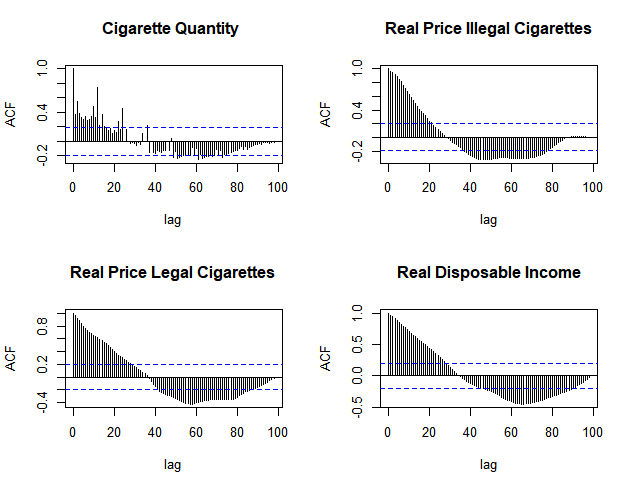
\includegraphics{img/ACF.png}
\caption{\label{plot2} ACF Plots}
\end{figure}

\begin{table}[H]
\centering
\begin{tabular}{lrll}
  \hline
Time Series & p value & Test Result & Interpretation \\ 
  \hline
Cigarette Quantity & 0.00 & Reject Null & Non-stationary \\ 
  Real Price Legal & 0.00 & Reject Null & Non-stationary \\ 
  Real Price Illegal & 0.00 & Reject Null & Non-stationary \\ 
  Real Disposable Income & 0.00 & Reject Null & Non-stationary \\ 
   \hline
\end{tabular}
\caption{Ljung-Box Test \label{box}} 
\end{table}

\begin{table}[H]
\centering
\begin{tabular}{lrll}
  \hline
Time Series & p value & Test Result & Interpretation \\ 
  \hline
Cigarette Quantity & 0.61 & Fail to reject Null & Non-stationary \\ 
  Real Price Legal & 0.22 & Fail to reject Null & Non-stationary \\ 
  Real Price Illegal & 0.38 & Fail to reject Null & Non-stationary \\ 
  Real Disposable Income & 0.06 & Fail to reject Null & Non-stationary \\ 
   \hline
\end{tabular}
\caption{Augmented Dickey-Fuller Test \label{adf}} 
\end{table}

To assess whether a long-run relationship between the variables exists,
the Johansen test is employed. According to Akaike's information
criterion (AIC), the appropriate maximum number of lags to use is 10
(\ref{lag}). A lag order of 9 is used for the test, since the test
requires a lag order of N - 1 = 10 - 1 = 9. Two Johansen tests are used:
the Trace and the Maximum Eigenvalue tests. The Trace statistic test
(\ref{coint}) shows we reject the null hypothesis that there are zero
cointegrating relationships: the test statistic 85.85 is greater than
the 1\% significance level of 55.43. The test results indicate that
there is 1 cointegrating relationship. Similarly, the Maximum Eigenvalue
test rejects that there are zero cointegrating relationships, and fails
to reject that there is at most 1 cointegrating relationship. The
presence of a cointegrating vector amongst the variables suggests a
Vector Error Correction Model is appropriate to analyse the variable
dynamics.

\begin{table}[H]
\centering
\begin{tabular}{rrrr}
  \hline
AIC(n) & HQ(n) & SC(n) & FPE(n) \\ 
  \hline
 10 &   5 &   2 &  10 \\ 
   \hline
\end{tabular}
\caption{Optimal Lag Selection \label{lag}} 
\end{table}

\begin{table}[H]
\centering
\begin{tabular}{rrrrr}
  \hline
 & Test Statistic & 10\% & 5\% & 1\% \\ 
  \hline
r$<$=3 & 1.21 & 6.50 & 8.18 & 11.65 \\ 
  r$<$=2 & 6.04 & 15.66 & 17.95 & 23.52 \\ 
  r$<$=1 & 26.89 & 28.71 & 31.52 & 37.22 \\ 
  r=0 & 85.85 & 45.23 & 48.28 & 55.43 \\ 
   \hline
\end{tabular}
\caption{Johansen Trace Test for Cointegration Results\label{coint}} 
\end{table}
\begin{table}[H]
\centering
\begin{tabular}{rrrrr}
  \hline
 & Test Statistic & 10\% & 5\% & 1\% \\ 
  \hline
r$<$=3 & 1.21 & 6.50 & 8.18 & 11.65 \\ 
  r$<$=2 & 4.83 & 12.91 & 14.90 & 19.19 \\ 
  r$<$=1 & 20.85 & 18.90 & 21.07 & 25.75 \\ 
  r=0 & 58.95 & 24.78 & 27.14 & 32.14 \\ 
   \hline
\end{tabular}
\caption{Johansen Eigenvalue Test for Cointegration Results\label{eigen}} 
\end{table}

\hypertarget{vector-error-correction-model}{%
\subsection{Vector Error Correction
Model}\label{vector-error-correction-model}}

A summary of the VECM results is given in \ref{vecm1}. The full model
output with the 9 lags is given in the appendix \ref{app}. The results
show that the error correction terms are not significant, with the
exception of the cigarette quantity term, and very few of the first lag
coefficients are significant.

\begin{longtable}{rll}
  \hline
 & ECT & Intercept \\ 
  \hline
QDP & -1.9701(0.5869)**  & 0.0054(0.0238)     \\ 
  PREALWAPDP & 0.0598(0.0301).   & -0.0022(0.0012).   \\ 
  PREALWAPDNP & -0.1659(0.1979)     & 0.0100(0.0080)     \\ 
  YDISPREAL & 0.0078(0.0081)     & 0.0001(0.0003)     \\ 
   \hline
\hline
\caption{Vector Error Correction Model 2OLS\label{vecm1}} 
\end{longtable}
\begin{longtable}{rllll}
  \hline
 & QDP-1 & PREALWAPDP-1 & PREALWAPDNP-1 & YDISPREAL-1 \\ 
  \hline
QDP & 0.7123(0.5286)     & -6.5487(2.6841)*   & 0.5219(0.5503)     & 12.7417(10.2110)     \\ 
  PREALWAPDP & -0.0565(0.0271)*   & 0.0007(0.1375)     & 0.0567(0.0282)*   & 0.9735(0.5229).   \\ 
  PREALWAPDNP & 0.1705(0.1783)     & 0.5743(0.9052)     & -0.2648(0.1856)     & -1.8064(3.4435)     \\ 
  YDISPREAL & -0.0078(0.0073)     & 0.0229(0.0369)     & 0.0093(0.0076)     & 0.8393(0.1406)*** \\ 
   \hline
\hline
\caption{Vector Error Correction Model 2OLS\label{vecm11}} 
\end{longtable}

To test the accuracy of the model, a number of diagnostic tests were
run. The majority of specification tests are modified for a Vector
Autoregression model (VAR) so first the results of the VECM were
converted to a VAR format. The Portmanteau serial correlation test shows
that the null hypothesis of no autocorrelation is rejected at a 1\%
level of significance since the p-value is 0. The ARCH test shows that
there are no ARCH effects (the test fails to reject the null). Finally,
the normality test indicates the the residuals of the VECM model are not
normally distributed. The serial correlation and normality test indicate
that the model could be better specified. The next section explores an
unstructured VAR model as an alternative.

\begin{table}[H]
\centering
\begin{tabular}{lrll}
  \hline
Test & p value & Test Result & Interpretation \\ 
  \hline
Portmanteau & 0.00 & Reject Null & Autorrelation \\ 
   \hline
\end{tabular}
\caption{Serial Correlcation Test \label{diag}} 
\end{table}
\begin{table}[H]
\centering
\begin{tabular}{lrll}
  \hline
Test & p value & Test Result & Interpretation \\ 
  \hline
ARCH & 1.00 & Fail to reject Null & No ARCH effects \\ 
   \hline
\end{tabular}
\caption{ARCH Tests \label{archh}} 
\end{table}
\begin{table}[H]
\centering
\begin{tabular}{lrll}
  \hline
Test & p value & Test Result & Interpretation \\ 
  \hline
Normality & 0.00 & Reject Null & Residuals not normally distributed \\ 
   \hline
\end{tabular}
\caption{Normality Tests \label{archh}} 
\end{table}

\hypertarget{unstructured-var}{%
\subsection{Unstructured VAR}\label{unstructured-var}}

If we proceed with using an unstructured VAR model despite the
non-stationarity of the time series, we get the base model below
(\ref{eq1}):

\begin{align}
 Q_t = \mu + \sum_{i = 1}^{n}\beta_iQ_{t-i} +\sum_{i = 1}^{n}\gamma_iP_{t-i} + \sum_{i = 1}^{n}\theta_iY_{t-i} + \sum_{i = 1}^{n}\phi_iI_{t-i} \label{eq1}
\end{align}

where \(Q_t\) is the log of cigarette consumption,\newline \(P_{t}\) is
the log of real cigarette price,\newline \(Y_{t}\) is the log of real
disposable income,\newline \(I_{t}\) is the log of real illicit
cigarette price,\newline \(n\) is the number of lags and t is measured
in months

The results of the VAR are presented in table \ref{varr} below. The
diagnostic tests are summarised in the tables under the regression
output in \ref{diagvar}. The VAR fairs better in the specification
tests, although there is stil serial correlation present.

\newpage

\begin{table}[!htbp] \centering 
  \caption{Vector Autoregression \label{varr}} 
  \label{} 
\footnotesize 
\begin{tabular}{@{\extracolsep{1pt}}lcccc} 
\\[-1.8ex]\hline 
\hline \\[-1.8ex] 
 & \multicolumn{4}{c}{\textit{Dependent variable:}} \\ 
\cline{2-5} 
\\[-1.8ex] & \multicolumn{4}{c}{y} \\ 
\\[-1.8ex] & (1) & (2) & (3) & (4)\\ 
\hline \\[-1.8ex] 
 Quantity.l1 & $-$0.424$^{***}$ (0.132) & $-$0.004 (0.007) & 0.003 (0.042) & $-$0.001 (0.002) \\ 
  Price.Duties.Paid.l1 & $-$5.153$^{*}$ (2.681) & 0.770$^{***}$ (0.132) & 0.649 (0.860) & $-$0.0005 (0.034) \\ 
  Price.Duties.not.Paid.l1 & 1.418$^{***}$ (0.450) & 0.019 (0.022) & 0.751$^{***}$ (0.144) & 0.004 (0.006) \\ 
  Disposable.Income.l1 & 5.829 (10.816) & 0.544 (0.532) & $-$2.093 (3.472) & 1.737$^{***}$ (0.138) \\ 
  Quantity.l2 & $-$0.122 (0.138) & $-$0.026$^{***}$ (0.007) & $-$0.010 (0.044) & $-$0.004$^{**}$ (0.002) \\ 
  Price.Duties.Paid.l2 & 3.291 (3.203) & $-$0.094 (0.158) & $-$0.763 (1.028) & $-$0.058 (0.041) \\ 
  Price.Duties.not.Paid.l2 & 0.088 (0.586) & $-$0.021 (0.029) & 0.306 (0.188) & 0.008 (0.008) \\ 
  Disposable.Income.l2 & 6.112 (21.486) & $-$0.940 (1.057) & $-$0.751 (6.896) & $-$0.584$^{**}$ (0.275) \\ 
  Quantity.l3 & $-$0.403$^{***}$ (0.128) & 0.005 (0.006) & $-$0.098$^{**}$ (0.041) & $-$0.001 (0.002) \\ 
  Price.Duties.Paid.l3 & $-$1.302 (3.132) & 0.340$^{**}$ (0.154) & 0.096 (1.005) & 0.004 (0.040) \\ 
  Price.Duties.not.Paid.l3 & $-$1.099$^{*}$ (0.584) & 0.054$^{*}$ (0.029) & 0.138 (0.187) & 0.002 (0.007) \\ 
  Disposable.Income.l3 & $-$28.207 (22.460) & 0.895 (1.105) & 9.412 (7.209) & $-$0.813$^{***}$ (0.287) \\ 
  Quantity.l4 & $-$0.178 (0.141) & 0.015$^{**}$ (0.007) & $-$0.126$^{***}$ (0.045) & 0.0004 (0.002) \\ 
  Price.Duties.Paid.l4 & 2.948 (3.139) & $-$0.181 (0.154) & 1.188 (1.007) & 0.029 (0.040) \\ 
  Price.Duties.not.Paid.l4 & 0.372 (0.562) & $-$0.027 (0.028) & 0.041 (0.180) & $-$0.007 (0.007) \\ 
  Disposable.Income.l4 & 17.786 (24.173) & $-$0.334 (1.190) & $-$10.458 (7.759) & 1.150$^{***}$ (0.309) \\ 
  Quantity.l5 & $-$0.132 (0.157) & 0.007 (0.008) & 0.145$^{***}$ (0.051) & $-$0.0001 (0.002) \\ 
  Price.Duties.Paid.l5 & $-$0.123 (3.180) & $-$0.062 (0.157) & $-$0.587 (1.021) & 0.010 (0.041) \\ 
  Price.Duties.not.Paid.l5 & $-$0.716 (0.564) & $-$0.045 (0.028) & $-$0.038 (0.181) & $-$0.017$^{**}$ (0.007) \\ 
  Disposable.Income.l5 & 3.474 (25.876) & $-$0.383 (1.274) & $-$1.791 (8.305) & $-$0.509 (0.331) \\ 
  Quantity.l6 & $-$0.356$^{**}$ (0.159) & $-$0.015$^{*}$ (0.008) & 0.069 (0.051) & 0.001 (0.002) \\ 
  Price.Duties.Paid.l6 & $-$3.564 (3.042) & $-$0.072 (0.150) & $-$0.559 (0.976) & 0.028 (0.039) \\ 
  Price.Duties.not.Paid.l6 & 0.032 (0.482) & 0.009 (0.024) & $-$0.163 (0.155) & 0.006 (0.006) \\ 
  Disposable.Income.l6 & $-$17.569 (23.169) & 0.052 (1.140) & 9.746 (7.436) & 0.049 (0.297) \\ 
  Quantity.l7 & $-$0.459$^{***}$ (0.166) & 0.009 (0.008) & $-$0.069 (0.053) & 0.001 (0.002) \\ 
  Price.Duties.Paid.l7 & 2.310 (2.887) & $-$0.056 (0.142) & 1.381 (0.927) & $-$0.045 (0.037) \\ 
  Price.Duties.not.Paid.l7 & 1.657$^{***}$ (0.473) & 0.010 (0.023) & $-$0.304$^{*}$ (0.152) & 0.005 (0.006) \\ 
  Disposable.Income.l7 & 8.108 (22.086) & $-$0.347 (1.087) & $-$8.990 (7.089) & $-$0.027 (0.283) \\ 
  Quantity.l8 & $-$0.375$^{**}$ (0.163) & $-$0.001 (0.008) & $-$0.060 (0.052) & $-$0.001 (0.002) \\ 
  Price.Duties.Paid.l8 & $-$1.022 (2.827) & 0.093 (0.139) & $-$0.947 (0.907) & $-$0.033 (0.036) \\ 
  Price.Duties.not.Paid.l8 & $-$0.571 (0.520) & $-$0.014 (0.026) & 0.303$^{*}$ (0.167) & $-$0.003 (0.007) \\ 
  Disposable.Income.l8 & 1.136 (20.760) & 1.055 (1.022) & 5.354 (6.663) & $-$0.095 (0.266) \\ 
  Quantity.l9 & $-$0.316$^{**}$ (0.151) & $-$0.010 (0.007) & $-$0.040 (0.048) & $-$0.003 (0.002) \\ 
  Price.Duties.Paid.l9 & 3.185 (2.367) & 0.049 (0.116) & $-$0.384 (0.760) & 0.007 (0.030) \\ 
  Price.Duties.not.Paid.l9 & 0.546 (0.459) & 0.018 (0.023) & $-$0.012 (0.147) & 0.007 (0.006) \\ 
  Disposable.Income.l9 & $-$0.681 (10.231) & $-$0.715 (0.504) & $-$0.717 (3.284) & 0.052 (0.131) \\ 
  const & 78.609$^{***}$ (25.524) & 3.378$^{***}$ (1.256) & 5.199 (8.192) & 0.807$^{**}$ (0.327) \\ 
 \hline \\[-1.8ex] 
Observations & 90 & 90 & 90 & 90 \\ 
R$^{2}$ & 0.826 & 0.984 & 0.979 & 1.000 \\ 
Adjusted R$^{2}$ & 0.708 & 0.973 & 0.965 & 0.999 \\ 
Residual Std. Error (df = 53) & 0.082 & 0.004 & 0.026 & 0.001 \\ 
F Statistic (df = 36; 53) & 7.007$^{***}$ & 90.623$^{***}$ & 68.995$^{***}$ & 3,434.504$^{***}$ \\ 
\hline 
\hline \\[-1.8ex] 
\textit{Note:}  & \multicolumn{4}{r}{$^{*}$p$<$0.1; $^{**}$p$<$0.05; $^{***}$p$<$0.01} \\ 
\end{tabular} 
\end{table}

\begin{table}[H]
\centering
\begin{tabular}{lrll}
  \hline
Test & p value & Test Result & Interpretation \\ 
  \hline
Portmanteau & 0.00 & Reject Null & Autorrelation \\ 
   \hline
\end{tabular}
\caption{Serial Correlcation Test \label{diagvar}} 
\end{table}
\begin{table}[H]
\centering
\begin{tabular}{lrll}
  \hline
Test & p value & Test Result & Interpretation \\ 
  \hline
ARCH & 1.00 & Fail to reject Null & No ARCH effects \\ 
   \hline
\end{tabular}
\caption{ARCH Tests \label{archh}} 
\end{table}
\begin{table}[H]
\centering
\begin{tabular}{lrll}
  \hline
Test & p value & Test Result & Interpretation \\ 
  \hline
Normality & 0.09 & Fail to reject Null & Residuals normally distributed \\ 
   \hline
\end{tabular}
\caption{Normality Tests \label{archhvar}} 
\end{table}

The results of the VAR are then used to calculate elasticities according
to the formula below:

\begin{equation}
\hat{E}_{d}=\frac{\sum_{t=1}^{9} \hat{\gamma}_{t}}{1-\sum_{t=1}^{9} \hat{\beta}_{t}}
\end{equation}

The elasticities are presented in the table below \ref{elastic}. The
income elasticity is expected to be positive; however, it is unusual
that both price elasticities are positive.

\begin{table}[H]
\centering
\begin{tabular}{lr}
  \hline
  \hline
Illicit price elasticity of cigarette demand & 0.27 \\ 
  Income elasticity & 0.26 \\ 
  Price elasticity & 0.21 \\ 
   \hline
\end{tabular}
\caption{Elasticities \label{elastic}} 
\end{table}

\hypertarget{discussion-points}{%
\section{\texorpdfstring{Discussion Points
\label{discuss}}{Discussion Points }}\label{discussion-points}}

There are several concerns that I have regarding the data work:

\begin{itemize}
\item
  How do I choose the appropriate maximum number of lags for the
  stationarity tests? Changing the max lags impacted the optimal lag
  selection results, which then changed some results from nonstationary
  to stationary.
\item
  If some of the time series are stationary and some are nonstationary,
  should I use a VECM or a VAR?
\item
  How do I interperet the coefficients of the VAR (and VECM) for the
  elasticities? I think this is where I am going wrong in my final
  calculations.
\end{itemize}

\newpage

\hypertarget{appendix}{%
\section*{\texorpdfstring{Appendix
\label{app}}{Appendix }}\label{appendix}}
\addcontentsline{toc}{section}{Appendix \label{app}}

The full model output for the VECM is given below (for all 9 lags):

\begin{verbatim}
##                                          ECT          Intercept
## Equation log_QDP          -1.9701(0.5869)**  0.0054(0.0238)    
## Equation log_PREALWAPDP    0.0598(0.0301).   -0.0022(0.0012).  
## Equation log_PREALWAPDNP -0.1659(0.1979)     0.0100(0.0080)    
## Equation log_YDISPREAL    0.0078(0.0081)     0.0001(0.0003)    
##                                   log_QDP -1  log_PREALWAPDP -1
## Equation log_QDP          0.7123(0.5286)     -6.5487(2.6841)*  
## Equation log_PREALWAPDP   -0.0565(0.0271)*   0.0007(0.1375)    
## Equation log_PREALWAPDNP  0.1705(0.1783)     0.5743(0.9052)    
## Equation log_YDISPREAL   -0.0078(0.0073)     0.0229(0.0369)    
##                           log_PREALWAPDNP -1     log_YDISPREAL -1
## Equation log_QDP          0.5219(0.5503)     12.7417(10.2110)    
## Equation log_PREALWAPDP    0.0567(0.0282)*      0.9735(0.5229).  
## Equation log_PREALWAPDNP -0.2648(0.1856)      -1.8064(3.4435)    
## Equation log_YDISPREAL    0.0093(0.0076)        0.8393(0.1406)***
##                                   log_QDP -2   log_PREALWAPDP -2
## Equation log_QDP           0.8721(0.4652).   -0.6078(2.7827)    
## Equation log_PREALWAPDP   -0.0746(0.0238)**  -0.1448(0.1425)    
## Equation log_PREALWAPDNP  0.1576(0.1569)     -0.7516(0.9384)    
## Equation log_YDISPREAL   -0.0088(0.0064)     -0.0246(0.0383)    
##                           log_PREALWAPDNP -2    log_YDISPREAL -2
## Equation log_QDP         -0.2354(0.5326)     5.1050(13.0520)    
## Equation log_PREALWAPDP   0.0185(0.0273)     -0.6844(0.6684)    
## Equation log_PREALWAPDNP  0.1521(0.1796)     -1.7708(4.4016)    
## Equation log_YDISPREAL     0.0144(0.0073).    0.1624(0.1797)    
##                                   log_QDP -3   log_PREALWAPDP -3
## Equation log_QDP          0.6822(0.4178)     -2.4916(2.5640)    
## Equation log_PREALWAPDP   -0.0543(0.0214)*     0.2848(0.1313)*  
## Equation log_PREALWAPDNP  0.0662(0.1409)     -0.3331(0.8647)    
## Equation log_YDISPREAL   -0.0082(0.0058)     -0.0257(0.0353)    
##                          log_PREALWAPDNP -3     log_YDISPREAL -3
## Equation log_QDP         -1.0656(0.4827)*   -22.5035(13.0477).  
## Equation log_PREALWAPDP   0.0716(0.0247)**    0.4249(0.6682)    
## Equation log_PREALWAPDNP 0.1933(0.1628)        7.6662(4.4001).  
## Equation log_YDISPREAL    0.0120(0.0066).     -0.6690(0.1796)***
##                                   log_QDP -4   log_PREALWAPDP -4
## Equation log_QDP           0.6858(0.3822).   -1.2043(2.5294)    
## Equation log_PREALWAPDP  -0.0315(0.0196)      0.1188(0.1295)    
## Equation log_PREALWAPDNP -0.0563(0.1289)      1.3067(0.8530)    
## Equation log_YDISPREAL   -0.0063(0.0053)      0.0114(0.0348)    
##                           log_PREALWAPDNP -4    log_YDISPREAL -4
## Equation log_QDP         -0.4782(0.4810)     2.7420(14.7493)    
## Equation log_PREALWAPDP   0.0192(0.0246)      0.3427(0.7553)    
## Equation log_PREALWAPDNP  0.1161(0.1622)     -4.4195(4.9739)    
## Equation log_YDISPREAL    0.0040(0.0066)       0.4683(0.2030)*  
##                                   log_QDP -5   log_PREALWAPDP -5
## Equation log_QDP           0.6104(0.3526).   -2.1442(2.4145)    
## Equation log_PREALWAPDP  -0.0198(0.0181)     -0.0097(0.1236)    
## Equation log_PREALWAPDNP  0.1164(0.1189)      0.7490(0.8142)    
## Equation log_YDISPREAL   -0.0050(0.0049)      0.0139(0.0332)    
##                           log_PREALWAPDNP -5    log_YDISPREAL -5
## Equation log_QDP          -1.1575(0.4806)*   8.4217(15.4113)    
## Equation log_PREALWAPDP  -0.0294(0.0246)     -0.6263(0.7892)    
## Equation log_PREALWAPDNP  0.0564(0.1621)     -6.3966(5.1972)    
## Equation log_YDISPREAL    -0.0116(0.0066).    0.0101(0.2121)    
##                                   log_QDP -6   log_PREALWAPDP -6
## Equation log_QDP          0.2154(0.3186)     -3.0998(2.3458)    
## Equation log_PREALWAPDP   -0.0275(0.0163).   -0.0928(0.1201)    
## Equation log_PREALWAPDNP   0.2134(0.1074).   -0.2221(0.7911)    
## Equation log_YDISPREAL   -0.0043(0.0044)       0.0570(0.0323).  
##                           log_PREALWAPDNP -6     log_YDISPREAL -6
## Equation log_QDP         -0.4884(0.4995)     -7.0755(14.3280)    
## Equation log_PREALWAPDP   0.0224(0.0256)       0.1192(0.7338)    
## Equation log_PREALWAPDNP -0.1171(0.1684)       4.9165(4.8319)    
## Equation log_YDISPREAL    0.0010(0.0069)       0.1489(0.1972)    
##                                   log_QDP -7   log_PREALWAPDP -7
## Equation log_QDP         -0.0028(0.2846)     -0.8281(2.4960)    
## Equation log_PREALWAPDP  -0.0136(0.0146)     -0.1651(0.1278)    
## Equation log_PREALWAPDNP  0.1221(0.0960)      0.8960(0.8417)    
## Equation log_YDISPREAL   -0.0028(0.0039)     -0.0009(0.0344)    
##                          log_PREALWAPDNP -7     log_YDISPREAL -7
## Equation log_QDP          0.7909(0.4494).   -9.3025(12.6131)    
## Equation log_PREALWAPDP  0.0218(0.0230)      -0.4428(0.6459)    
## Equation log_PREALWAPDNP -0.3807(0.1516)*    -4.6557(4.2536)    
## Equation log_YDISPREAL   0.0061(0.0062)      -0.0462(0.1736)    
##                                   log_QDP -8   log_PREALWAPDP -8
## Equation log_QDP         -0.0038(0.2306)     -0.9364(2.3362)    
## Equation log_PREALWAPDP  -0.0157(0.0118)      0.0052(0.1196)    
## Equation log_PREALWAPDNP  0.0144(0.0778)      0.1434(0.7878)    
## Equation log_YDISPREAL   -0.0019(0.0032)     -0.0085(0.0322)    
##                           log_PREALWAPDNP -8     log_YDISPREAL -8
## Equation log_QDP         -0.5773(0.4488)     -2.5085(12.5567)    
## Equation log_PREALWAPDP  -0.0024(0.0230)       0.4481(0.6431)    
## Equation log_PREALWAPDNP -0.0005(0.1514)       0.2502(4.2345)    
## Equation log_YDISPREAL   -0.0017(0.0062)      -0.0958(0.1728)    
##                                   log_QDP -9   log_PREALWAPDP -9
## Equation log_QDP         -0.1666(0.1414)       5.0666(2.2707)*  
## Equation log_PREALWAPDP   -0.0160(0.0072)*    0.1370(0.1163)    
## Equation log_PREALWAPDNP -0.0262(0.0477)     -1.1288(0.7657)    
## Equation log_YDISPREAL   -0.0030(0.0019)     -0.0382(0.0313)    
##                           log_PREALWAPDNP -9   log_YDISPREAL -9
## Equation log_QDP          -1.1384(0.4241)**  2.1330(9.8460)    
## Equation log_PREALWAPDP   0.0234(0.0217)     0.1289(0.5042)    
## Equation log_PREALWAPDNP  0.1289(0.1430)     0.0685(3.3204)    
## Equation log_YDISPREAL   -0.0039(0.0058)     0.0162(0.1355)
\end{verbatim}

\bibliography{Tex/ref}





\end{document}
